\documentclass[ngerman]{presentation}
\setlength{\fboxsep}{0mm}
\newmintedfile{ada}{autogobble,frame=lines,linenos,mathescape,framesep=2mm,breaklines,fontsize=\scriptsize}
\newmint{ada}{autogobble,mathescape}
\newmintinline{ada}{autogobble,mathescape}
\newminted{ada}{autogobble,mathescape,breaklines,fontsize=\scriptsize}
\newmintedfile{c}{autogobble,frame=lines,linenos,mathescape,framesep=2mm,breaklines,fontsize=\scriptsize}
\newmint[ci]{c}{autogobble,mathescape}
\newmintinline{c}{autogobble,mathescape}
\newminted{c}{autogobble,mathescape,breaklines,fontsize=\scriptsize}
\newmintedfile{rest}{autogobble,frame=lines,linenos,mathescape,framesep=2mm,breaklines,fontsize=\scriptsize}
\newmint{rest}{autogobble,mathescape}
\newmintinline{rest}{autogobble,mathescape}
\newminted{rest}{autogobble,mathescape,breaklines,fontsize=\scriptsize}

% Pfad für Eingabedateien
\makeatletter
\def\input@path{{chapters/}}
\makeatother
\graphicspath{{./images/},{../uml/build/}}

% ----------------------------------------------
\title{\textbf{Simulation von Echtzeit-Prozessen in Ada und C/POSIX}}
\subtitle{Projektarbeit}
\author{Jan Strohbeck}
\institute[Hochschule Aalen] {
	Studiengang Informatik (Master of Science)\\
	Hochschule Aalen - Technik und Wirtschaft
}
\date{14.\ März 2017}

\begin{document}

\maketitle
\newpage

% ----------------------------------------------
\begin{frame}{\contentsname}
\tableofcontents
\end{frame}

% - Übersicht
\section{Übersicht}
\label{sec:uebersicht}

% Übersicht
\begin{frame}[c,label=uebersicht]
    \frametitle{Übersicht}

    Ziel der Arbeit: Erstellung von Simulationen für zwei Echtzeit-Umgebungen,
    jeweils in Ada und C/POSIX, für die Vorlesung \enquote{Echtzeitsysteme}.

    Umgebungen:

    \begin{itemize}
        \item Druck- und Temperatursteuerung
        \item Parkplatz
    \end{itemize}

    Außerdem:
    \begin{itemize}
        \item Erstellung einer Dokumentation zur Verwendung der Umgebungen für
            Studenten
        \item Parametrierbare Ausgabe der Simulation
    \end{itemize}
\end{frame}

% ----------------------------------------------
% - Druck- und Temperatursteuerung
\section{Druck- und Temperatursteuerung}
\label{sec:druck-_und_temperatursteuerung}

% -- Übersicht
\subsection{Übersicht}
\label{sec:uebersicht}

% Übersicht
\begin{frame}[c,label=uebersicht]
    \frametitle{Übersicht}

    \begin{center}
    \includegraphics[width=\textwidth]{simple_embedded_system_overview}
    \end{center}
\end{frame}

% --- Interface
\subsubsection{Interface}
\label{sec:interface}


% Interface
\begin{frame}[c,label=interface]
    \frametitle{Interface}
    \hspace*{-0.9cm}\includegraphics[width=1.15\textwidth]{simple_embedded_system_interface}
\end{frame}

% -- Realisierung
\subsection{Realisierung}
\label{sec:realisierung}

% Realisierung
\begin{frame}[c,label=realisierung]
    \frametitle{Realisierung}

    \begin{itemize}
        \item Temperatur nimmt ab, wenn keine Heizung an ist
        \item Temperatur nimmt zu, wenn Heizung an ist
            \pause
        \item Druck nimmt proportional ab, wenn Einstellung $<$ 0
        \item Druck nimmt proportional zu, wenn Einstellung $>$ 0
        \item Druck verändert sich nicht, wenn Einstellung $=$ 0
    \end{itemize}

    \pause

    \begin{itemize}
        \item Convert-Funktionen beinhalten simple Regelung auf einen Sollwert
            (20 Grad Celsius, 1000 mbar)
    \end{itemize}
\end{frame}

% Realisierung
\begin{frame}[c,label=realisierung]
    \frametitle{Realisierung}

    \hspace*{-0.9cm}\includegraphics[width=1.15\textwidth]{simple_embedded_system_simulators}
\end{frame}

% Realisierung
\begin{frame}[c,label=realisierung]
    \frametitle{Realisierung}

    \textbf{Ada}:
    \begin{itemize}
        \item Protected Objects
        \item Tasks
        \item Modularisierung über Ada-Packages, \adainline!package body!
    \end{itemize}

    \pause

    \textbf{C/POSIX}:
    \begin{itemize}
        \item Mutexe
        \item Threads
        \item Modularisierung über C/Header-Files, \cinline!static!-Variablen
    \end{itemize}
\end{frame}

% ----------------------------------------------
\section{Parkplatz}
\label{sec:parkplatz}

% -- Übersicht
\subsection{Übersicht}
\label{sec:uebersicht}

% Übersicht
\begin{frame}[c,label=uebersicht]
    \frametitle{Übersicht}

    \vspace{-0.6cm}\hspace*{-0.8cm}\includegraphics[width=1.15\textwidth]{parking_lot_overview}
\end{frame}

% -- Interface
\subsection{Interface}
\label{sec:interface}

% Interface
\begin{frame}[c,label=interface]
    \frametitle{Interface}

    \hspace*{-0.9cm}\includegraphics[width=1.15\textwidth]{parking_lot_interface}
\end{frame}

% -- Realisierung
\subsection{Realisierung}
\label{sec:realisierung}

% Realisierung
\begin{frame}[c,label=realisierung]
    \frametitle{Realisierung}

    \begin{itemize}
        \item Autos entscheiden zufällig, ob sie den Parkplatz betreten möchten
            (oder verlassen möchten, falls sie bereits drin sind)
        \item Autos müssen sich in eine Warteschlage einreihen zum Betreten oder
            Verlassen
        \item Autos können die Warteschlage verlassen wenn sie nicht innerhalb
            einer bestimmten Zeit eingelassen werden
    \end{itemize}
\end{frame}

% Realisierung
\begin{frame}[c,label=realisierung]
    \frametitle{Realisierung}

    \vspace{-0.6cm}\hspace*{-0.9cm}\includegraphics[width=1.15\textwidth]{parking_lot_simulators}
\end{frame}

% Realisierung
\begin{frame}[c,label=realisierung]
    \frametitle{Realisierung}

    \textbf{Ada}:
    \begin{itemize}
        \item Protected Objects
        \item Tasks
        \item Ada-Rendezvous zwischen Tasks mit Abbruchmöglichkeit
        \item Modularisierung über Ada-Packages, \adainline!package body!
    \end{itemize}

    \pause

    \textbf{C/POSIX}:
    \begin{itemize}
        \item Mutexe
        \item Condition Variables
        \item Semaphoren
        \item Threads
        \item Modularisierung über C/Header-Files, \cinline!static!-Variablen
    \end{itemize}
\end{frame}

% ----------------------------------------------
\section{Dokumentation}
\label{sec:dokumentation}

% Dokumentation
\begin{frame}[c,label=dokumentation]
    \frametitle{Dokumentation}

    \vspace{-0.6cm}
    \begin{center}
    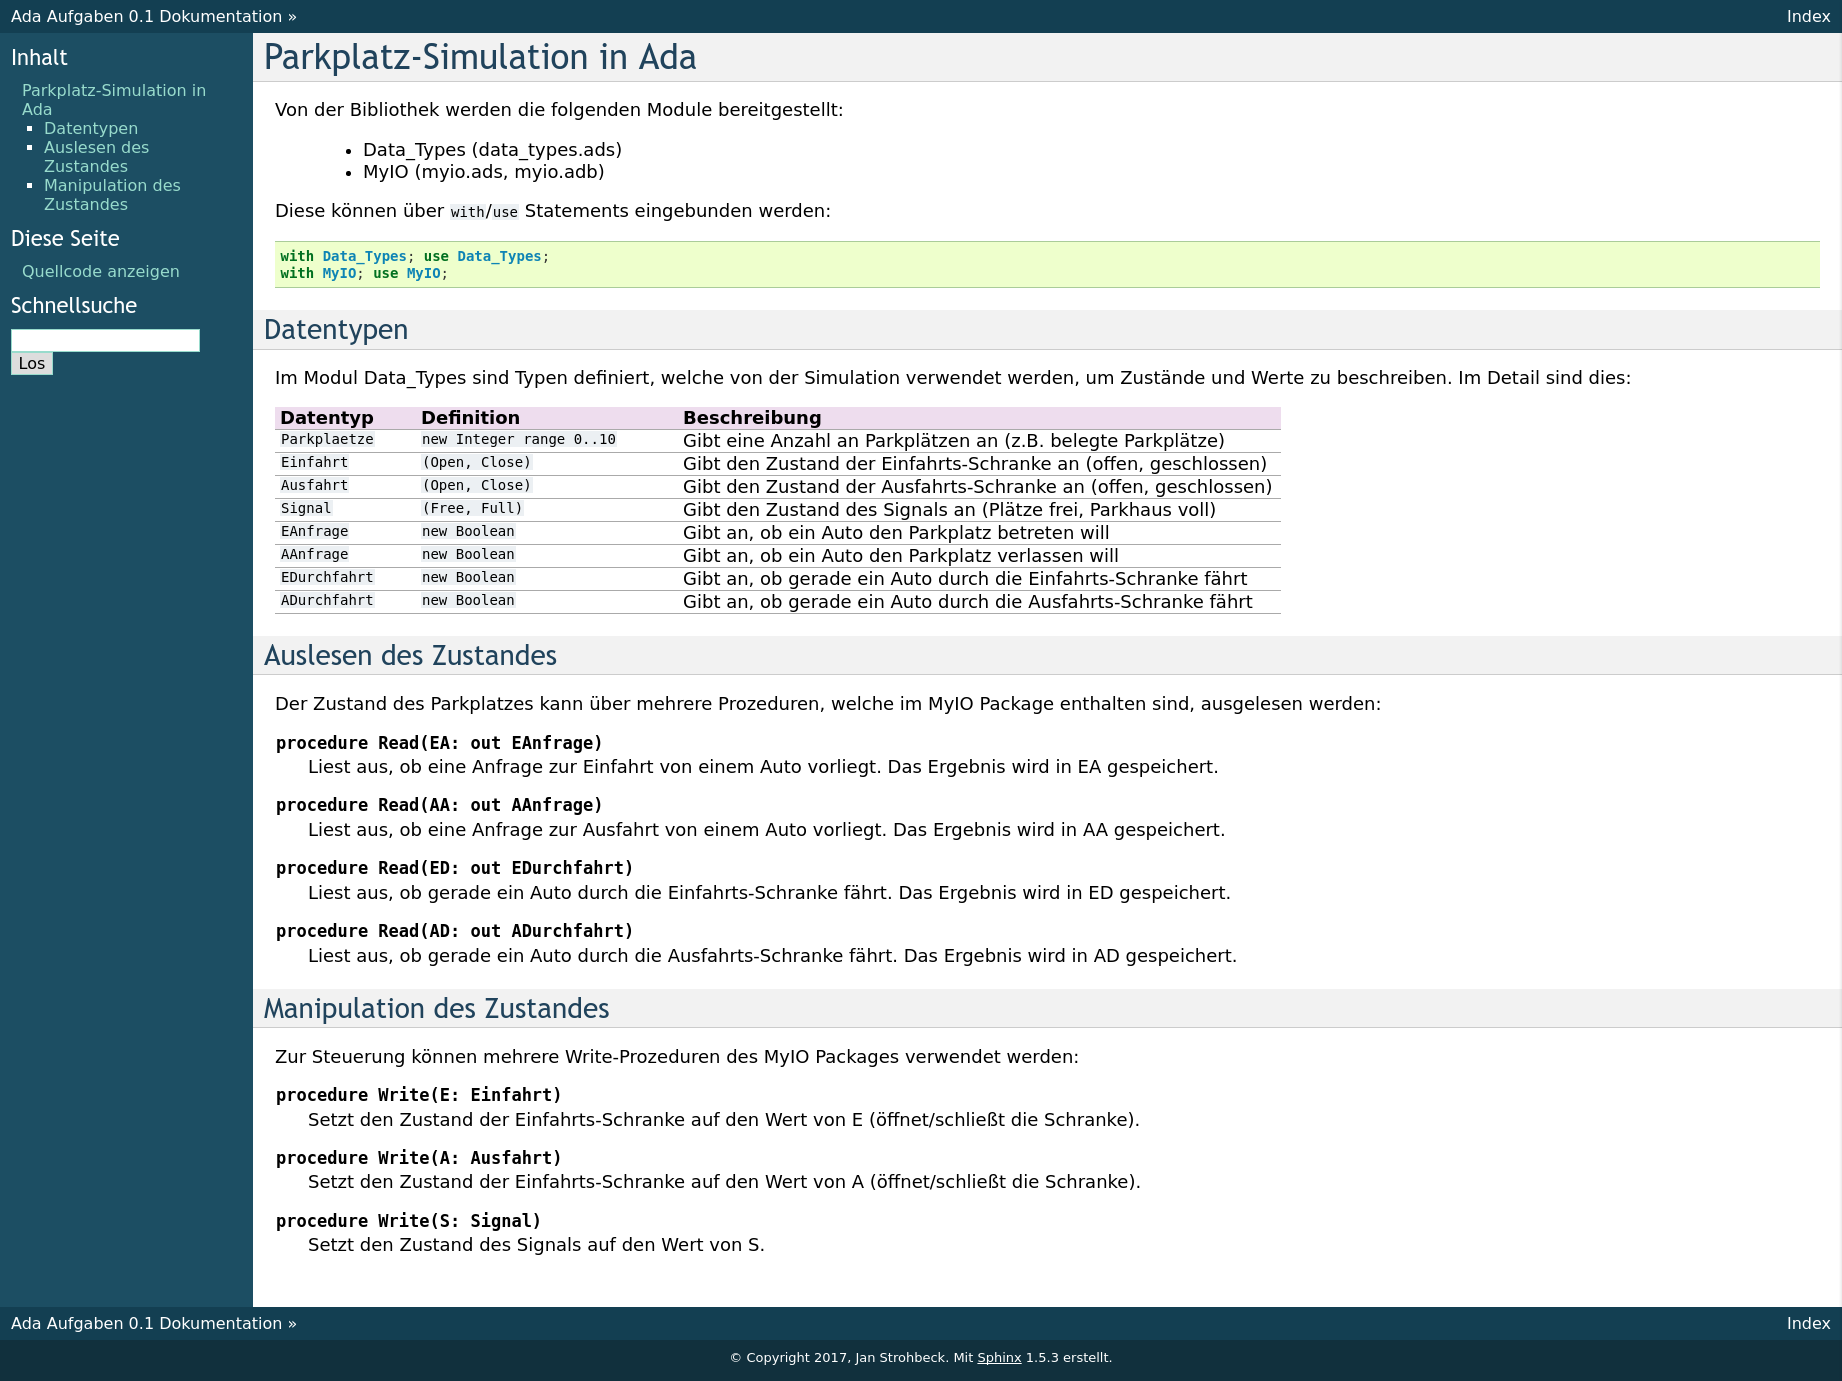
\includegraphics[width=0.96\textwidth]{sphinx_doc}
    \end{center}
\end{frame}

% --- Sphinx
\subsubsection{Sphinx}
\label{sec:sphinx}

% Sphinx
\begin{frame}[c,label=sphinx,fragile]
    \frametitle{Sphinx}
    
    Dokumentation mithilfe von reStructuredText:

    \begin{quote}
        \normalfont
        \begin{restcode}
            Parkplatz-Simulation in Ada
            ===========================

            .. highlight:: ada

            Von der Bibliothek werden die folgenden Module bereitgestellt:

             - Data_Types (data_types.ads)
             - MyIO (myio.ads, myio.adb)

            Diese können über ``with``/``use`` Statements eingebunden werden::

               with Data_Types; use Data_Types;
               with MyIO; use MyIO;
        \end{restcode}
    \end{quote}
\end{frame}

% - Aktueller Status
\section{Aktueller Status}
\label{sec:aktueller_status}

% Aktueller Status
\begin{frame}[c,label=aktueller_status]
    \frametitle{Aktueller Status}

    \begin{itemize}
        \item Programmierung abgeschlossen
        \item Stellenweise noch Refactoring notwendig
        \item Dokumentation noch unvollständig
    \end{itemize}
\end{frame}

% ----------------------------------------------
%\section*{Referenzen}
%\begin{frame}[allowframebreaks]
%\begin{scriptsize}
%\raggedright\printbibliography
%\end{scriptsize}
%\end{frame}

% ----------------------------------------------
\section*{}
\begin{frame}
\centering\huge\textbf{Live-Demo}
\end{frame}

% Ablauf
\begin{frame}[c,label=ablauf]
    \frametitle{Ablauf}

    \vspace{-0.6cm}
    \begin{center}
    \includegraphics[height=0.85\textheight]{parking_lot_requestqueue}
    \end{center}
\end{frame}

% --- Timeout
\subsubsection{Timeout}
\label{sec:timeout}

% Timeout
\begin{frame}[c,label=timeout]
    \frametitle{Timeout}

    \vspace{-0.6cm}
    \begin{center}
    \includegraphics[height=0.85\textheight]{parking_lot_requestqueue_timeout}
    \end{center}
\end{frame}
% ----------------------------------------------
\end{document}
